\begin{figure}[ht]
\centering
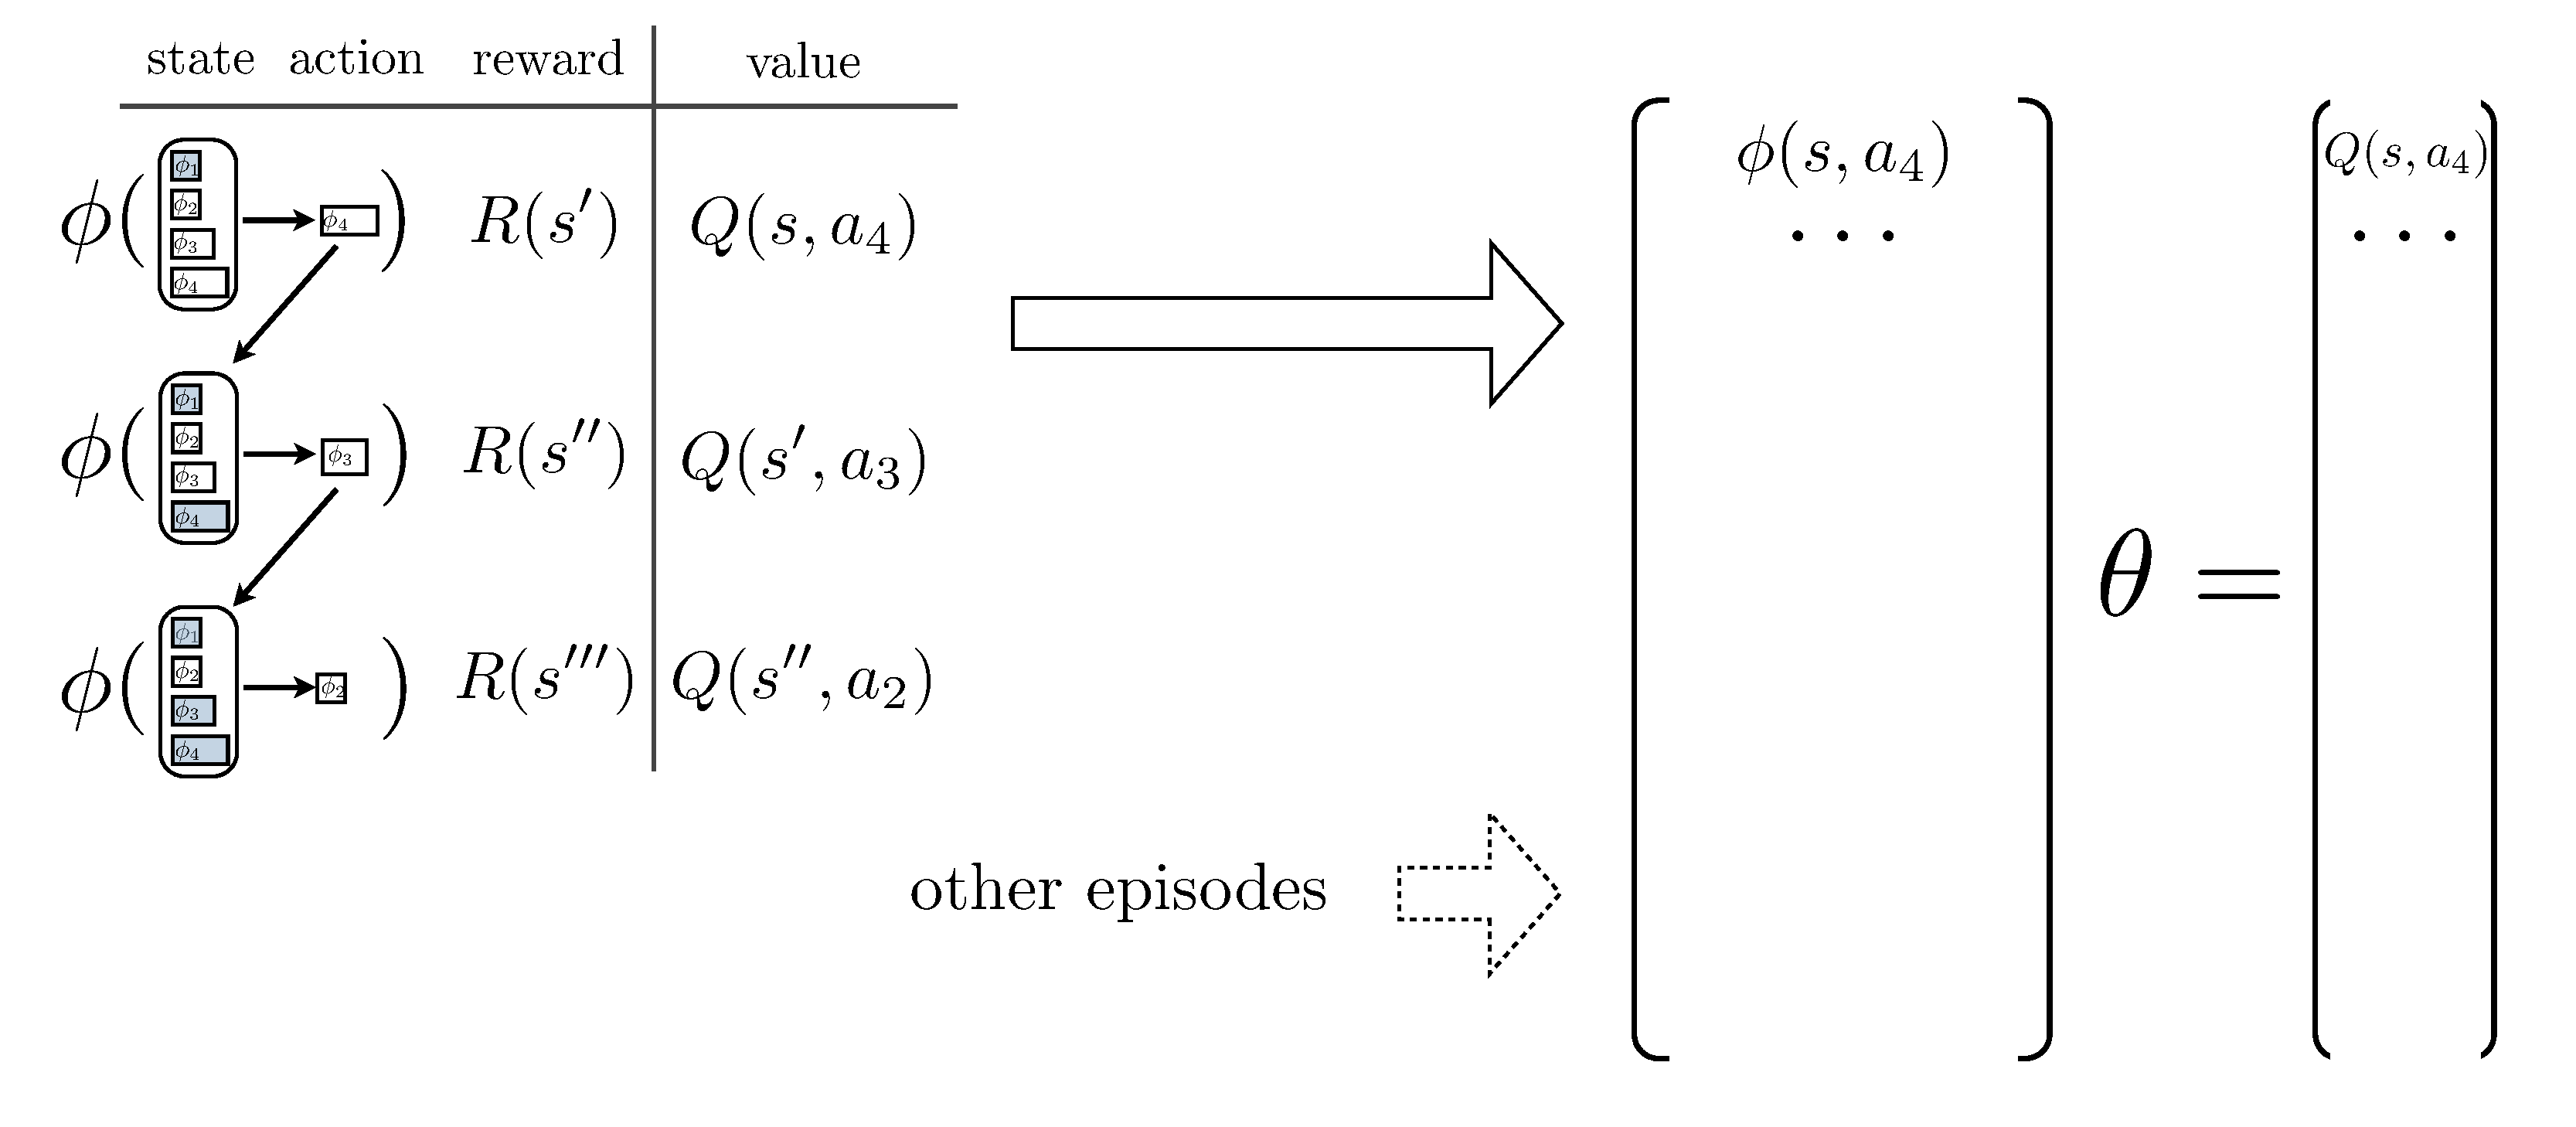
\includegraphics[width=\linewidth]{../../figures/qiteration_explanation.pdf}
\caption[
Explanation of the Q-iteration method.]{
We sample $Q^\pi(s, a) = \mathbb{E}_{s'} \left[ R(s') + \gamma Q^\pi(s', \pi(s')) \right] = \theta^T \phi(s, a)$ by running the policy over many images.
Once an episode is complete, the $Q$-value at each $(s, a)$ can be determined.
To update the policy, simply minimize the prediction error of $\theta$, and repeat.
\label{fig:qiteration_explanation}}
\end{figure}
